\documentclass[a4paper,11pt]{article}

% ---------- Packages ----------
\usepackage[margin=2.5cm]{geometry}
\usepackage{amsmath, amssymb, amsthm, mathtools}
\usepackage{algorithm}
\usepackage{algpseudocode}
\usepackage{enumitem}
\usepackage{graphicx}
\usepackage{booktabs}
\usepackage{hyperref}
\usepackage{xcolor}

\usepackage{tikz}
\usetikzlibrary{automata,positioning,arrows.meta}

% ---------- Theorem Environments ----------
\newtheorem{theorem}{Theorem}
\newtheorem{lemma}{Lemma}
\newtheorem{definition}{Definition}
\newtheorem{proposition}{Proposition}
\newtheorem{corollary}{Corollary}

% ---------- Custom Commands ----------
\newcommand{\R}{\mathbb{R}}
\newcommand{\N}{\mathbb{N}}
\newcommand{\Z}{\mathbb{Z}}
\newcommand{\Alphabet}{\Sigma}
\newcommand{\eps}{\varepsilon}
\newcommand{\set}[1]{\left\{ #1 \right\}}
\newcommand{\abs}[1]{\left| #1 \right|}
\newcommand{\ceil}[1]{\left\lceil #1 \right\rceil}
\newcommand{\floor}[1]{\left\lfloor #1 \right\rfloor}

% ---------- Section Style ----------
\renewcommand{\thesubsection}{(\alph{subsection})}
\renewcommand{\thesection}{}

% ---------- Algorithm Style ----------
\algrenewcommand\algorithmicrequire{\textbf{Input:}}
\algrenewcommand\algorithmicensure{\textbf{Output:}}

% ---------- Title Info ----------
\title{\textbf{CSE2315 --- Assignment 4}}
\author{Vlad Paun \\ 6152937}
\date{\today}

% ---------- Document ----------
\begin{document}

	\maketitle

	\section{Exercise 1}
	Old exam question, endterm 2022--2023: Given the Turing Machine $M$ below. You may assume the tape is bounded on the left.

	You may assume that any missing transitions lead to the reject state, which has been left out.

	\begin{center}
		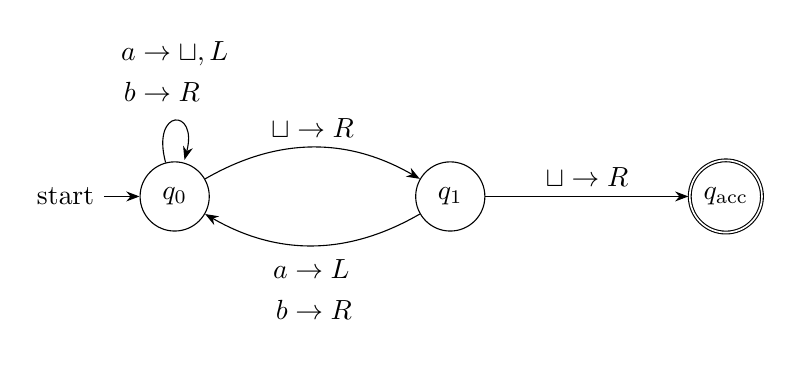
\begin{tikzpicture}[->, >=Stealth, auto, node distance=3.5cm]
			\node[initial,state] (q0) {$q_0$};
			\node[state] (q1) [right of=q0] {$q_1$};
			\node[accepting,state] (qacc) [right of=q1] {$q_{\mathrm{acc}}$};

			\path
			(q0) edge[bend left] node[above] {$\sqcup \to R$} (q1)
			(q1) edge[bend left] node[below] {$\begin{aligned}
					a & \to L\\
					b &\to R
				\end{aligned}$} (q0)
			(q0) edge[loop above] node {$\begin{aligned}
					a &\to \sqcup,L \\
					b &\to R
				\end{aligned}$} (q0)
			(q1) edge node {$\sqcup \to R$} (qacc);
		\end{tikzpicture}
	\end{center}

	\subsection{Give two words that are in $L(M)$ and two words that are not. For at least one of each, explain why not by giving the sequence of configurations the machine goes through. All words should be at least length 2.}
	\begin{align*}
		bba,bbb&\in L(M)\\
		& q_0bba,bq_0ba,bbq_0a,bq_0b,bbq_0,bb\sqcup q_1,bb\sqcup\sqcup q_{acc}\\
		bbaa,baa&\notin L(M)
	\end{align*}


	\subsection{Describe the language $L(M)$ (you can do this informally or in set-builder notation).}
	The language consists of all words with no 2 consecutive $a$'s in it

	\subsection{Is $L(M)$ decidable? Explain your answer.}
	It is not decidable as it loops forever when it encounters 2 consecutive $a$'s.

	\section{Exercise 2}
	Suppose we have the following language over the alphabet $\Alphabet = \set{1,\dots,9,\#}$:
	\[
	L = \set{v\#w \mid v,w \in \set{1,\dots,9}^* \land \exists a,b \in \set{1,\dots,9} : c_a(v) = c_b(w)}
	\]
	where $c_x(y)$ denotes the number of occurrences of symbol $x$ in word $y$.

	Give a high-level description of a nondeterministic Turing machine that decides $L$.

	On input $x$:
	\begin{enumerate}
		\item Check the format.\\
		Verify that $x$ has exactly one symbol $\#$ and all other symbols are in $\set{1,\dots,9}$
		\item Split the input as $a\#b$
		\item Nondeterministically guess the two digits $a$ and $b$
		\item count the number of $a$'s in $v$ and $b$'s in $w$ by matching them
		\item When there are no more unmarked $a$'s, if there are any unmarked $b$'s left, reject, otherwise accept
	\end{enumerate}


	\section{Exercise 3}
	Suppose we have the following language over the alphabet $\Alphabet = \set{0,1,\#}$:
	\[
	L = \set{0^n\#1^m \mid n > m}
	\]

	Describe an order in which we can enumerate $L$. Does your order show that $L$ is decidable?

	An order in which we can enumerate $L$ is the following:
	\begin{itemize}
		\item Start with the word $0\#$ and print it
		\item While the $\#$ is at index 1 + midpoint of the word, replace the symbol before the $\#$ with a $\#$ and replace the original $\#$ with a $1$ and print it
		\item When the $\#$ reaches the midpoint of the word, overwrite all characters of the word with $0$ and then append a $\#$ and go back to the rule above
	\end{itemize}

	The language is decidable as the enumerator enumerates in shortlex order, in order to decide on a word, we just wait until the enumerator either enumerates it or goes past the length of the word.

	\section{Exercise 4}
	Consider the following language:
	\[
	L = \set{\langle v_1,v_2,\dots,v_k,D\rangle \mid v_1,v_2,\dots,v_k \in \set{0,1}^* \text{ and $D$ is a DFA with } L(D)=\bar{K},\text{ where }K=\set{v_1,v_2,\dots,v_k}}
	\]

	Is the following Turing machine $M$ a decider for $L$? Explain.

	\begin{quote}
		$M =$ ``On input $w = \langle v_1,v_2,\dots,v_j,D\rangle$:
		\begin{enumerate}[label=\arabic*.]
			\item For $i = 1,\dots,j$:
			\begin{enumerate}[label=\alph*.]
				\item Run $D$ on $v_i$.
				\item If $D$ accepts, reject.
			\end{enumerate}
			\item If $D$ has rejected all $v_i$, accept.''
		\end{enumerate}
	\end{quote}
	No it does not. The machine only checks if the DFA D rejects all $v_i$, but it does not check that D accepts all words in $\set{0,1}^*-K$.

	\section{Exercise 5}
	Old exam question, resit 22--23.

	\subsection{Given a Turing Machine $M$ with input alphabet $\Alphabet$ and tape alphabet $\Gamma$. Is it possible for $|\Gamma| = |\Alphabet| + 2$? If yes, draw a valid TM $M$ for which this holds. If not, explain why not.}
	Yes, it is possible. The input alphabet has to be a subset of the tape alphabet, as the tape must at least contain the $\sqcup$ symbol. More than that, the tape alphabet can contain any number of symbols that do not appear in the input one. For example, using a special $\$$ symbol for marking stuff for example

	\vspace{1cm}

	\subsection{Can a Turing Machine contain just a single state? If yes, draw a valid Turing Machine with a single state. If not, explain why not.}
	No, as a Turing machine must have exactly one accepting and one rejecting distinct states.

	\vspace{1cm}

	\section{Exercise 6}
	Revision, old exam question midterm 18--19: Consider the following language, where the alphabet $\Alphabet = \set{a,b}$:
	\[
	L = \set{b^n a b v \mid v \in \Alphabet^*,\ n \geq 1,\ \text{and } |v| = 8n + 4}
	\]

	This language is not regular. Prove this using the pumping lemma in at most 20 lines.

	\begin{proof}
		By contradiction.\\
		Assume for the sake of contradiction that the language $L$ is regular. Let $p$ be the pumping length given by the pumping lemma. Choose $s$ to be the string $b^pabv$. Because $s$ is a member of $L$ and has length more than $p$, the pumping lemma guarantees that $s$ can be split into three pieces, $s = xyz$, where for any $i \ge 0$ the string $xy^iz$ is in $L$. We show this outcome is impossible.\\
		Condition 3 of the pumping lemma says that $|xy| \le p$. Thus, in the case of our word, y must consist of only $b$s. $xyyz$ would therefore be $b^{2n}abv$, but $|v|\neq 8(2n) + 4$, so $xyyz$ is not in L. Therefore, $s$ cannot be pumped, which is a contradiction.
	\end{proof}

	\section{Exercise 7}
	Revision, variation on old exam question midterm 20--21:

	Given the GNFA $G$ depicted below. If we rip $q_2$ out of $G$ using the procedure described in Sipser, what non-empty transitions would be left in $G$? Make sure to describe all transitions.

	\begin{center}
		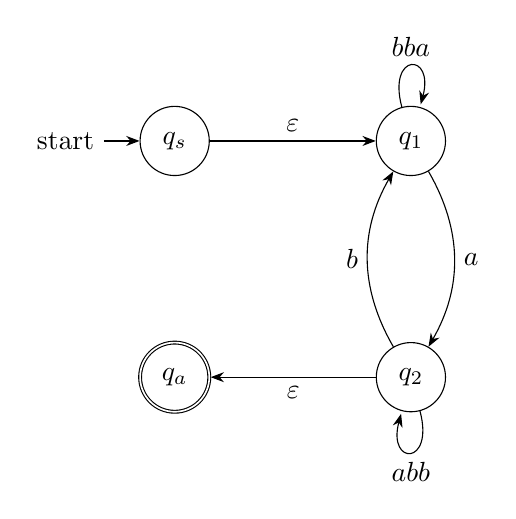
\begin{tikzpicture}[->, >=Stealth, auto, node distance=3cm]
			\node[initial,state] (qs) {$q_s$};
			\node[state] (q1) [right of=qs] {$q_1$};
			\node[state] (q2) [below of=q1] {$q_2$};
			\node[accepting,state] (qa) [below of=qs] {$q_a$};

			\path
			(qs) edge node {$\eps$} (q1)
			(q1) edge[loop above] node {$bba$} (q1)
			(q1) edge [bend left]node {$a$} (q2)
			(q2) edge [bend left]node {$b$} (q1)
			(q2) edge [loop below] node {$abb$} (q2)
			(q2) edge node {$\eps$} (qa);
		\end{tikzpicture}
	\end{center}



	\begin{center}
		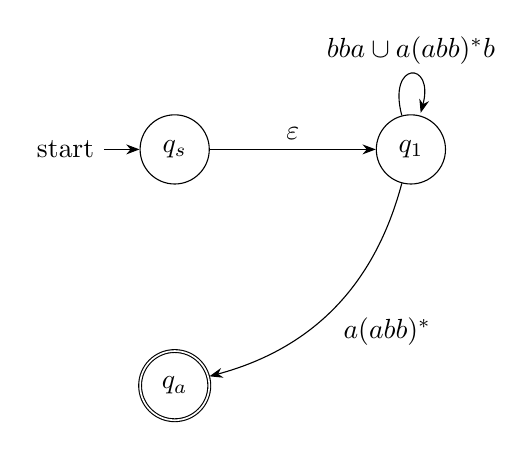
\begin{tikzpicture}[->, >=Stealth, auto, node distance=3cm]
			\node[initial,state] (qs) {$q_s$};
			\node[state] (q1) [right of=qs] {$q_1$};

			\node[accepting,state] (qa) [below of=qs] {$q_a$};

			\path
			(qs) edge node {$\eps$} (q1)
			(q1) edge[loop above] node {$bba\cup a(abb)^*b$} (q1)
			(q1) edge [bend left]node {$a(abb)^*$} (qa);

		\end{tikzpicture}
	\end{center}

	\section{Bonus Exercise}

\end{document}